%!TEX root = vorlage.tex

\section{Discussion}\label{sec:discussion}

Fully Convolutional Networks are also in this domain clearly superior to
traditional approaches. However, examining results such as the one shown
in~\cref{fig:fcn-result}, one can see that there is room for improvement. While
the overall position was correctly detected and the proposal is fairly
consistent, the model fails to match borders exactly. Simple improvements such
as combining the results of a FCN with the baseline might already fix this
problem. More elaborate techniques such as Conditional Random Fields (CRFs) are
also promising.

\begin{figure}[ht]
    \centering
    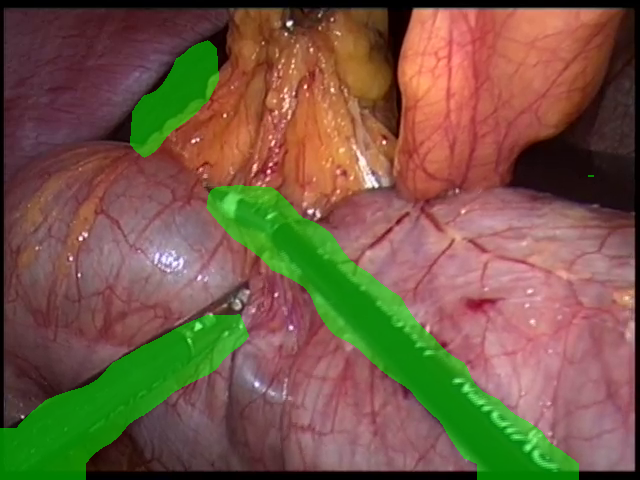
\includegraphics[width=\linewidth]{images/7-img_07.png}
    \caption{Semantic segmentation result of the FCN. While it }
    \label{fig:fcn-result}
\end{figure}
